\documentclass[presentation,mathserif,9pt]{beamer}


\usepackage{adjustbox}
\usepackage{algorithm}
\usepackage{algpseudocode}
\usepackage{amsfonts}
\usepackage{amsmath}
\usepackage{amssymb}
\usepackage{amsthm}
\usepackage{array}
\usepackage{blindtext}
\usepackage{cite}
\usepackage{cuted}
\usepackage{caption}
\usepackage{environ}
\usepackage{graphicx}
\usepackage{grffile}
\usepackage{hyperref}
\usepackage{import}
\usepackage{lmodern}
\usepackage{mathtools}
\usepackage{microtype}
\usepackage{multirow}
\usepackage{pgfgantt}
\usepackage{pgfplots}
\usepackage{physics}
\usepackage{setspace}
\usepackage{siunitx}
\usepackage{stfloats}
\usepackage{subcaption}
\usepackage{tikz}
\usepackage{url}
\usepackage{xcolor}
\usepackage[acronym]{glossaries-extra}
\usepackage[font=footnotesize,labelfont=bf]{caption}
\usepackage[RPvoltages]{circuitikz}
\usepackage[T1]{fontenc}
\usepackage[short]{optidef}

% tikz/pgf
\pgfplotsset{compat=newest}
\usetikzlibrary{plotmarks}
\usetikzlibrary{arrows.meta}
\usepgfplotslibrary{patchplots}

% amsthm
\newtheorem{proposition}{Proposition}

% siunitx
\DeclareSIUnit{\belmilliwatt}{Bm}
\DeclareSIUnit{\dBm}{\deci\belmilliwatt}

% caption
\captionsetup[figure]{labelformat=empty}

% footnote
\setbeamerfont{footnote}{size=\tiny}

% glossaries-extra
\setabbreviationstyle[acronym]{long-short}
\newacronym{af}{AF}{Amplify-and-Forward}

\usetheme{Warsaw}
\setbeamertemplate{page number in head/foot}[totalframenumber]
\setbeamertemplate{bibliography item}{\insertbiblabel}
\title[Semantic Communications: An Introduction]{\LARGE{\textbf{Semantic Communications: An Introduction}}}
\subtitle{Group Presentation}
\author{Yang Zhao}
\institute{Department of Electrical and Electronic Engineering\\Imperial College London}
\date{\today}

% ! error may due to losses in any source coding, noise in the channel, or their combinations.
% ! different background knowledge or inference rules, memories, feedbacks
% ! the presence of background knowledge reduces the informativeness of the source; However, if the background knowledge is shared, the reduction in semantic entropy means that we can compress the source without losing information: source information is the same amount, but can be compressed based on receiver's knowledge
% ? transmitter and receiver should 1) have some shared (e.g., file type) and local knowledge (e.g., purpose), which can be ``of higher level''; 2) the message generator has great freedom in picking a ``good'' code: accurate, easy to generate, destination interested in (redundancy and reliability).
% ? background can be memory- or learning-based results, some semantic communication is enabled even if no physical channel
% ! there is still a gap between visual features and semantics
% * example on dog classification: why not classify at tx and transmit result only? local knowledge, how much content to transmit for just right decision?
% ! why deep learning?
\begin{document}

\begin{frame}
	\titlepage
\end{frame}

\begin{frame}{Table of Contents}
	\tableofcontents
\end{frame}

\begin{section}{Theory}
	\begin{subsection}{Background and Intuitions}
		\begin{frame}{Shannon's Information Theory}
			\begin{figure}
				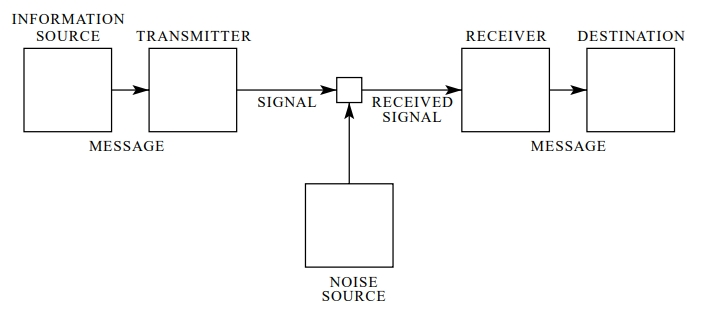
\includegraphics[width=0.6\textwidth]{assets/engineering_communication_system.jpg}
				\caption{Schematic diagram of an engineering/technical communication system \cite{Shannon1948}.}
			\end{figure}
			\begin{exampleblock}{A Mathematical Theory of Communication \cite{Shannon1948}\hspace*\fill--- C. E. Shannon}
				The fundamental problem of communication is that of reproducing at one point either exactly or approximately a message selected at another point. Frequently the messages have \alert{\emph{meaning;}} that is they refer to or are correlated according to some system with certain physical or conceptual entities. \alert{These semantic aspects of communication are irrelevant to the engineering problem.}
				% \hspace*\fill{\small--- C. E. Shannon}
			\end{exampleblock}
			\singlespacing
			Did Shannon intentionally excluded semantics from information theory?
			% ! communications from engineering perspective (Shannon) and everyday perspective
		\end{frame}

		\begin{frame}{Three Levels of Communications}
			\begin{figure}
				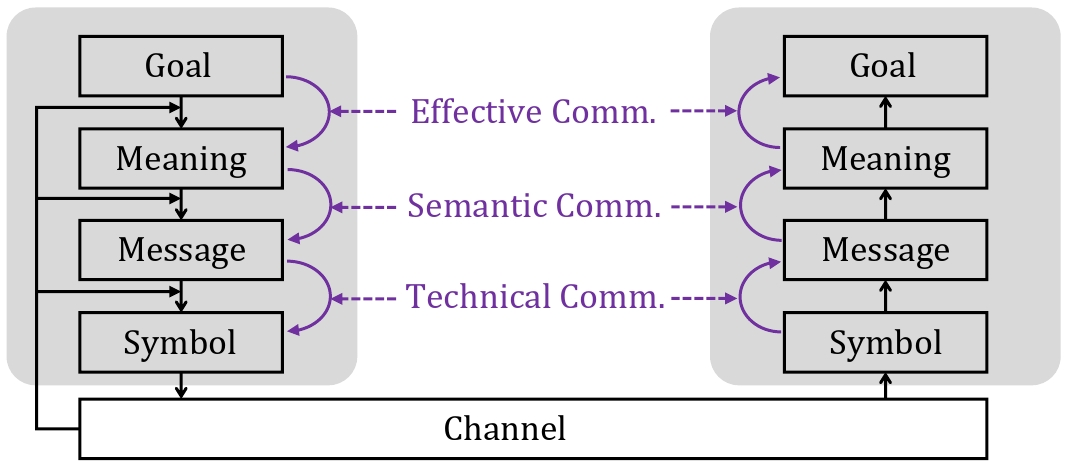
\includegraphics[width=0.6\textwidth]{assets/broad_communication_process.jpg}
				\caption{A broad communication process with three levels \cite{Shao2022}.}
			\end{figure}
			\begin{exampleblock}{Three Levels of Communications \cite{Weaver1953}\hspace*\fill--- W. Weaver}
				\begin{itemize}
					\item Level A. How accurately can the symbols of communication be transmitted? (The \alert{technical} problem.)
					\item Level B. How precisely do the transmitted symbols convey the desired meaning? (The \alert{semantic} problem.)
					\item Level C. How effectively does the received meaning affect conduct in the desired way? (The \alert{effectiveness} problem.)
				\end{itemize}
				% \hspace*\fill{\small--- W. Weaver}
			\end{exampleblock}
		\end{frame}

		\begin{frame}{Communication Problems}
			\begin{figure}
				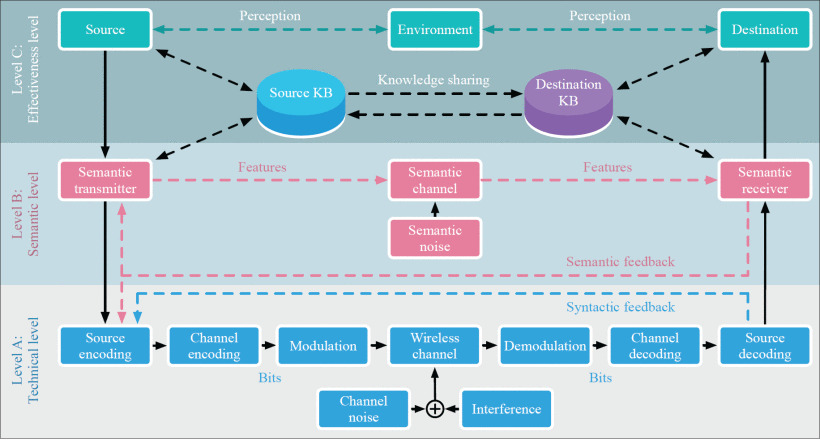
\includegraphics[width=0.7\textwidth]{assets/three_level_communication_model.jpg}
				\caption{A three-level communication model \cite{Luo2022a}; KB means ``knowledge base''.}
			\end{figure}
			\vspace{-0.4cm}
			\begin{block}{Communication Problems}
				\begin{itemize}
					\item \textbf{Technical communication:} design symbols for accurate message \emph{reconstruction} at the receiver as possible.
					\item \textbf{\color{blue}Semantic communication:} construct the right message to accurately convey the \emph{meaning} based on the agreed language;
					\item \textbf{Effective communication:} generate the right meaning for the ultimate \emph{goal}, under the states of the transmitter, receiver, and the progress of the task.
				\end{itemize}
			\end{block}
		\end{frame}

		\begin{frame}{What is Semantics?}
			\begin{figure}
				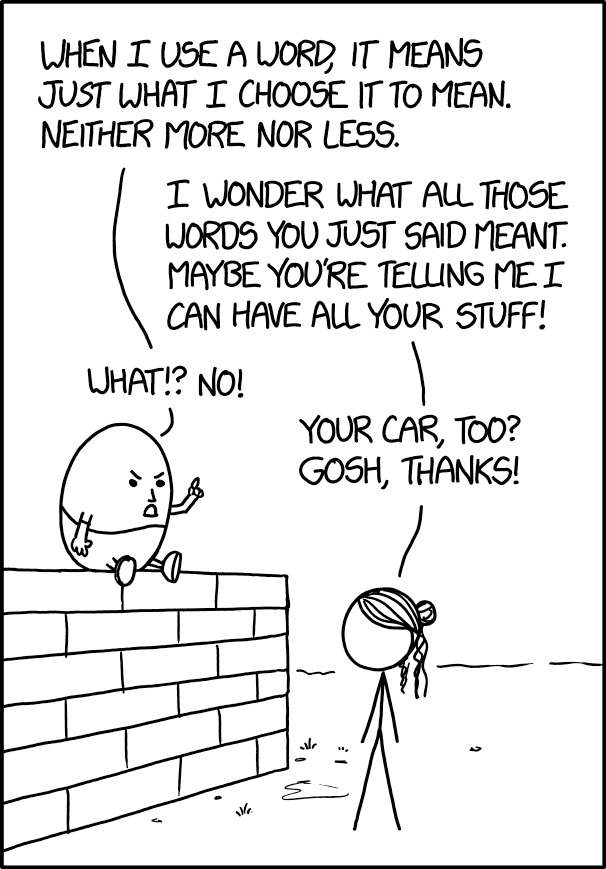
\includegraphics[width=0.275\textwidth]{assets/xkcd.jpg}
				\footnote[frame]{``Communicating'' by xkcd is licensed under CC BY-NC 2.5. Source: https://xkcd.com/1860/}
			\end{figure}
			\vspace{-0.2cm}
			\begin{alertblock}{Semantics Deals With `Meaning' \cite{Weaver1953}\hspace*\fill--- W. Weaver}
				The semantic problems are concerned with the interpretation of meaning by the receiver, as compared with the intended meaning of the sender.
			\end{alertblock}
			\vspace{-0.125cm}
			\begin{itemize}
				\item Formal or mathematical definition is difficult
				\item Many attempts from the perspective of \emph{logic} or \emph{word} rather than \emph{statistics}
				\item Cares about the delivery of meaning, not symbol-level reconstruction
			\end{itemize}
			% * examples: Apple
			% ! engineering failure and semantic failure
		\end{frame}

		\begin{frame}{Semantic Source and Destination}
			% * as you can imagine, semantic source 1) try to convey some meaning 2) can encode meaning in some form (e.g., bits, text, audio, video)
			A semantic source ...
			% can emit messages using a given syntax, such that these messages are ``true'' in the source, based on its state and inference capabilities.
			\begin{itemize}
				\item has the ability to \emph{observe, judge} and encode
				\item believes the statement is ``true'' w.r.t. its observations and experience
				\item expects the destination to ``understand'' the message to some degree
			\end{itemize}
			A semantic destination ...
			\begin{itemize}
				\item has the ability to \emph{observe, judge} and decode
				\item draws conclusions from the received message and the local knowledge
			\end{itemize}
			\begin{exampleblock}{Example: What is This?}
				\begin{figure}
					
\includegraphics[width=0.2\textwidth]{assets/duolingo.png}
					\footnote[frame]{For non-profit use in the context. Duolingo logo is an intellectual property of Duolingo, Inc.}
				\end{figure}
			\end{exampleblock}
			% ! semantic world: every thing (message) is absolutely true or false
			% ! semantic source has freedom to pick a ``good'' code: accurate, easy-to-generate, interesting, elegant... (redundancy and reliability)
		\end{frame}

	\end{subsection}

	\begin{subsection}{Semantic Information Theory}
		\begin{frame}{Semantic Source and Destination}
			Formally, a semantic source/receiver is a tuple $(W_{s/r}, K_{s/r}, I_{s/r}, M_{s/r})$
			\begin{itemize}
				\item $W_{s/r}$ is the model of worlds potentially observable by the source/receiver;
				\item $K_{s/r}$ is the background knowledge base of the source/receiver;
				\item $I_{s/r}$ is the inference procedure used by the source/receiver;
				\item $M_{s/r}$ is the message generator/interpreter (i.e., semantic encoder/decoder).
			\end{itemize}
			\begin{figure}
				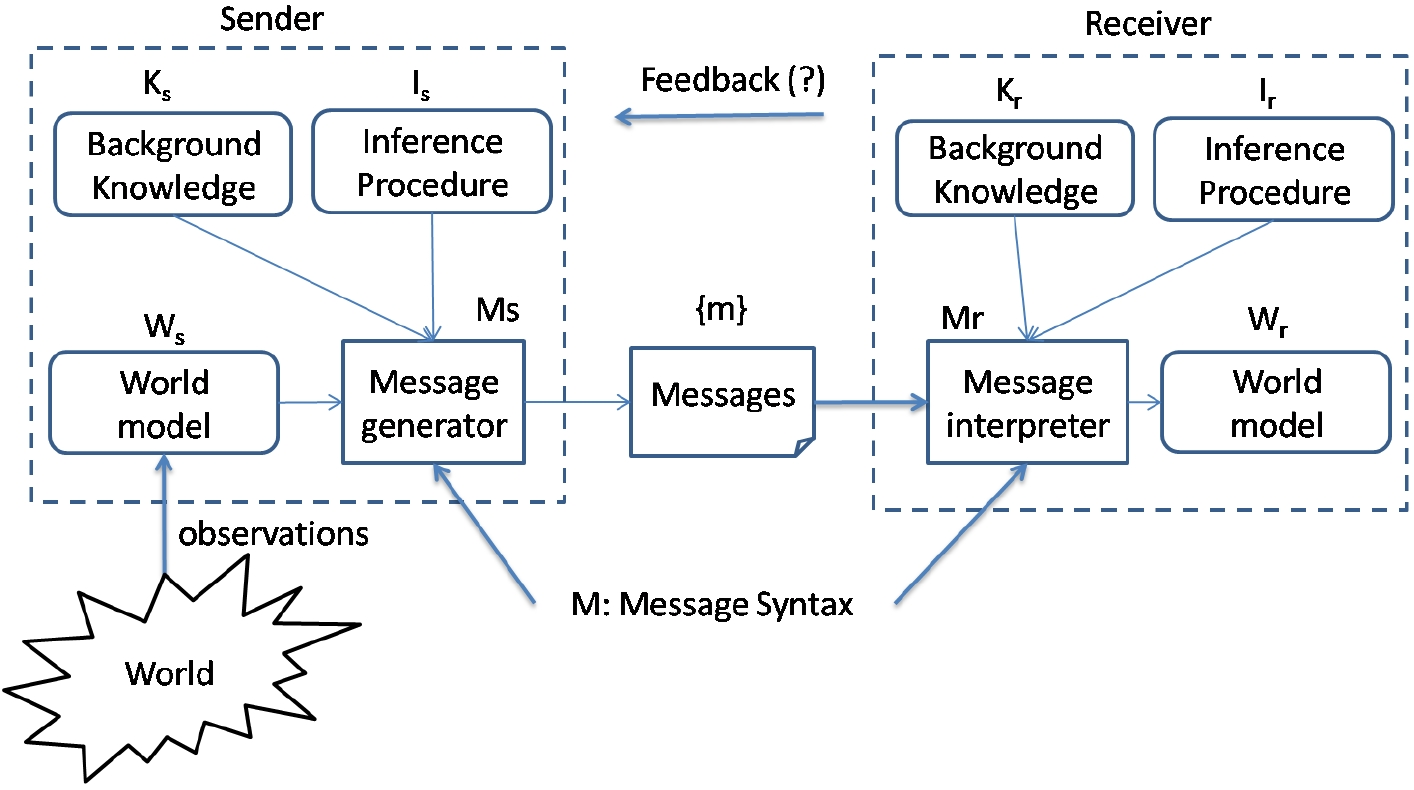
\includegraphics[width=0.6\textwidth]{assets/semantic_source_and_destination.jpg}
				\caption{Semantic source and destination \cite{Bao2011}}
			\end{figure}
			\vspace{-0.2cm}
			Possible outputs of the message generator can be seen as an interface language $X$ for the source.
			% ! transmitter and receiver becomes higher level (task- or human-oriented), with conventional transmitter and receiver as subsystem
		\end{frame}

		\begin{frame}{The Concept of Semantic Information}
			\begin{alertblock}{Amount of (Semantic) Information}
				\begin{itemize}
					\item In Shannon's theory \cite{Shannon1948}, the information of a message is governed by its \alert{statistical probability} but not its meaning (e.g., whether the message itself is true or false).
					\item In Carnap and Bar-Hillel's theory \cite{Carnap1952}, the semantic information of a message is determined by its \alert{logical probability} under their language system, but not the frequency of codewords.
				\end{itemize}
			\end{alertblock}

			\begin{exampleblock}{Example: Amount of (Semantic) Information in a Sentence}
				\vspace{0.1cm}
				\begin{enumerate}
					\item Kelly is a PhD student.
					\item Kelly is a postgraduate student.
				\end{enumerate}
				\vspace{0.1cm}
				\small{Sentence 2 has more Shannon information based on the \emph{statistical distribution} of English words (``PhD'' is more common than ``postgraduate''). However, sentence 1 has more semantic information because, according to their \emph{meanings and logical relationship}, doctor student is a subset of postgraduate student.}
			\end{exampleblock}
		\end{frame}

		\begin{frame}{Model Entropy}
			The {\color{blue} model entropy} of the semantic source is defined as
			\begin{equation}
				H(W) = - \sum_{w} \mu(w) \log_2 \mu(w)
			\end{equation}
			\vspace{-0.3cm}
			\begin{itemize}
				\item $w \in W$ is an interpretation of world model $W$ with probability $\mu(w)$.
				\item If the semantic source becomes the technical source with symbol set $W$, model entropy $H(W)$ becomes the Shannon entropy.
			\end{itemize}
		\end{frame}

		\begin{frame}{Logical Probability and Semantic Entropy}
			The {\color{blue} logical probability} of a message (sentence) $x \in X$ generated by $M$ is
			\begin{equation}
				m(x) = \frac{\mu(W_x)}{\mu(W)} = \frac{\sum_{w \models x} \mu(w)}{\sum_{w} \mu(w)}
			\end{equation}
			\vspace{-0.3cm}
			\begin{itemize}
				\item $w \models x$ reads $w$ models $x$, or that sentence $x$ is satisfied by observation $w$.
				\item $W_x = \{w \in W \mid w \models x\}$ is the model set of message $x$.
				\item $m(x)$ denotes the probability of message $x$ being true (over interpretations to the world model).
				\item When $W$ is not constrained by the background knowledge, $\sum_{w} \mu(w)=1$.
			\end{itemize}
			\singlespacing
			The {\color{blue} semantic entropy} of a message $x$ is
			\begin{equation}
				H_s(x) = -\log_2 m(x)
			\end{equation}
			\vspace{-0.3cm}
			\begin{itemize}
				\item There is no {\color{gray}background knowledge}
				\item Propositions are {\color{gray}independent} of each other
			\end{itemize}
		\end{frame}

		\begin{frame}{Conditional Entropy and Background Knowledge Base}
			When there is a background knowledge base $K$, the possible worlds are restricted to the subset of $W$ that is compatible with $K$
			\begin{align}
				m(x \mid K)   & = \frac{\sum_{w \models K, x} \mu(w)}{\sum_{w \models K} \mu(w)} \\
				H_s(x \mid K) & = -\log_2 m(x \mid K)
			\end{align}

			Let $\mu'$ be the new distribution of world models when $K$ is present, then
			\begin{align}
				\mu'(w)     & = \frac{\mu(w)}{\sum_{w' \models K} \mu(w')}  \\
				H(W \mid K) & = - \sum_{w \models K} \mu'(w) \log_2 \mu'(w)
			\end{align}
		\end{frame}

		\begin{frame}{Background Knowledge Base}
			\begin{exampleblock}{Example: Background Knowledge}
				Suppose $p(A)=p(B)=1/2$, $A$ and $B$ are independent propositions, and the background knowledge is $K=\{A \to B\}$ ($K$ is false iff $A$ is true and $B$ is false).
				\begin{table}[]
					\begin{tabular}{|c|c|c|c|}
						\hline
						$A$ & $B$ & {\color{blue} $A \to B$} & Probability \\ \hline
						0   & 0   & {\color{blue} 1}         & 1/4         \\ \hline
						0   & 1   & {\color{blue} 1}         & 1/4         \\ \hline
						1   & 0   & {\color{blue} 0}         & 1/4         \\ \hline
						1   & 1   & {\color{blue} 1}         & 1/4         \\ \hline
					\end{tabular}
				\end{table}
				The conditional logical probabilities are \emph{different} from statistical probabilities due to the presence of background knowledge
				\begin{equation*}
					m(A \mid K) = 1/3, \quad m(B \mid K) = 2/3, \quad m(A \wedge B \mid K) = 1/3,
				\end{equation*}
				where $A$ and $B$ are no longer logically independent!
				The mode entropies of the source without and with background knowledge are
				\begin{align*}
					H(W)        & = -4 \times 1/4 \log_2 1/4 = 2     \\
					H(W \mid K) & = -3 \times 1/3 \log_2 1/3 = 1.585
				\end{align*}
			\end{exampleblock}
		\end{frame}

		\begin{frame}{Background Knowledge Base: Good or Bad?}
			Q: Does the presence of background knowledge {\color{gray} reduces} the informativeness of the source?
			\singlespacing
			A: This is true when the source {\color{gray} does not share} background knowledge with the destination. However, if the background knowledge is {\color{blue} shared}, the reduction in semantic entropy means that we can {\color{blue} compress} the source without losing information!
			% * examples: common stream, CSIT
		\end{frame}

		\begin{frame}{Semantic Source Coding}
			\singlespacing
			\begin{alertblock}{Semantic Source Coding}
				For a given interface language, semantic source coding\footnote[frame]{As will be discussed later, semantic source and channel coding have different goals, and they are jointly called semantic coding.} needs to achieve two potentially conflicting goals:
				\begin{itemize}
					\item Maximizing expected faithfulness in representing the observed worlds (be \alert{authentic});
					\item Minimizing expected coding length (be \alert{precise}).
				\end{itemize}
			\end{alertblock}
			\singlespacing
			\begin{exampleblock}{Examples: Use of Language}
				\begin{itemize}
					\item ``Greater than or equal to'' can be coded as ``no smaller than''
					\item ``Mon$\vee$Tue$\vee$Wed$\vee$Thu$\vee$Fri'' can be coded as ``weekday''
				\end{itemize}
			\end{exampleblock}
		\end{frame}

		\begin{frame}{Semantic Coding: Discussion}
			A {\color{blue} semantic coding} strategy is a conditional probabilistic distribution $P(X \mid W)$.
			\singlespacing
			The distribution of message $x$ and Shannon entropy of interface language $X$ are
			% \begin{align}
			% 	P(x) & = \sum_{w} \mu(w) P(x \mid w) \\
			% 	H(X) & = -\sum_{x} P(x) \log_2 P(x)
			% \end{align}
			\begin{equation}
				P(x) = \sum_{w} \mu(w) P(x \mid w), \quad H(X) = -\sum_{x} P(x) \log_2 P(x)
			\end{equation}
			\vspace{-0.3cm}
			\begin{block}{Message Entropy and Model Entropy}
				\begin{equation}
					\underbrace{H(X)}_{\text{message entropy}} = \underbrace{H(W)}_{\text{model entropy}} + \underbrace{H(X \mid W) - H(W \mid X)}_{\text{can be } >, <, = 0}
				\end{equation}
				\vspace{-0.3cm}
				\begin{itemize}
					\item $H(X \mid W)$ measures {\color{blue} semantic redundancy} of the coding.
					\item $H(W \mid X)$ measures {\color{blue} semantic ambiguity} of the coding.
				\end{itemize}
				The message entropy can be larger or smaller than model entropy, depending on whether redundancy or ambiguity is larger.
			\end{block}
			\begin{exampleblock}{Examples: Compression and Explanation}
				\begin{itemize}
					\item $H(X) < H(W)$: presentation of a paper, use of abbreviations, etc.
					\item $H(X) > H(W)$: interpretation of a formula, use of examples, etc.
				\end{itemize}
			\end{exampleblock}
			% ! interpretation of a formula, presentation of a paper,
		\end{frame}

		\begin{frame}{Engineering and Semantic Channel}
			% ! A key difference between engineering communication and semantic communication is how infidelity is handled.
			\begin{figure}
				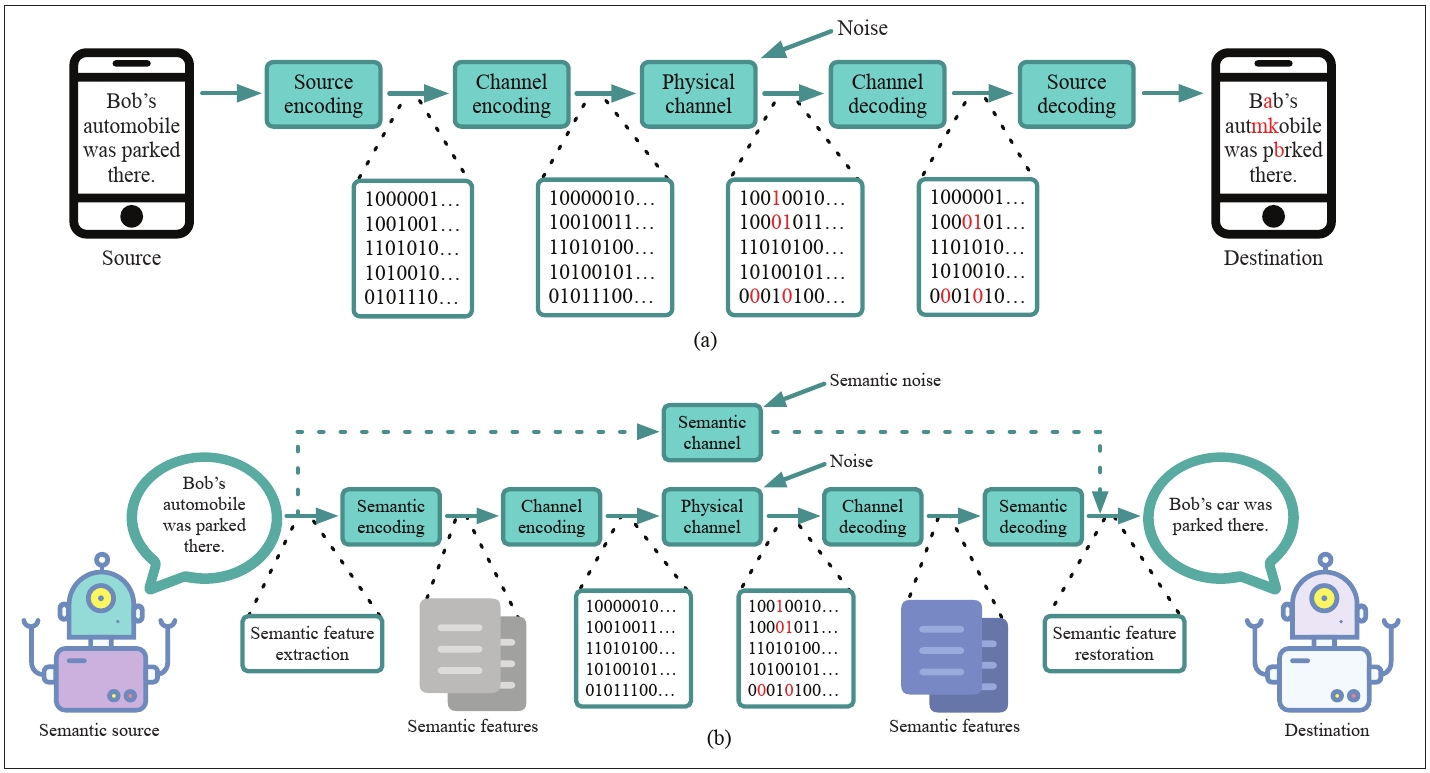
\includegraphics[width=0.9\textwidth]{assets/engineering_and_semantic_communications.jpg}
				\caption{Engineering and semantic communication systems \cite{Luo2022a}.}
			\end{figure}
			\begin{itemize}
				\item Engineering: a mapping from input to output is either a match or not.
				\item Semantic: concerned with semantic similarity between input and output.
			\end{itemize}
			% ! Some kind of duality: engineering message is general while semantic message is either true or false.
		\end{frame}

		\begin{frame}{Semantic Noise}
			% ! Semantic communication is at higher level of communications.
			Noise in semantic communication may be added at engineering and/or semantic level(s).
			There are two kinds of semantic errors:
			\begin{itemize}
				\item Unsoundness: the sent message is true but the received message is false, i.e., $w \models x$ but $w \not\models y$.
				\item Incompleteness: the sent message is false but the received message is true, i.e., $w \not\models x$ but $w \models y$.
			\end{itemize}

			% * Example: reader may error in few letters
			\begin{exampleblock}{Not all syntactic errors will lead to semantic errors (vise versa)}
				\begin{itemize}
					\item Readers maay undrestand the meaing of this sentense.
					\item h-bar is too small.
				\end{itemize}
			\end{exampleblock}
		\end{frame}

		\begin{frame}{Semantic Channel Coding}
			\begin{alertblock}{Semantic Channel Coding}
				For a given observed world, semantic channel coding aims to choose the strategy that can best tolerate noise (minimize unsoundness), or equivalently
				\begin{equation}
					\max \sum_{w \models y} p(w,x,y)
				\end{equation}
			\end{alertblock}
			% The goal of semantic channel coding is to minimize unsoundness, or equivalently
			% \vspace{-0.3cm}
			\begin{itemize}
				\item $p(w,x,y)=p(y \mid w,x)p(w,x)=p(y \mid x)p(w,x)$
				\item $p(w,x)=p(x \mid w)\mu(w)$
			\end{itemize}
			\singlespacing
			That is,
			\begin{equation}
				\max \sum_{w \models y} \underbrace{p(y \mid x)}_{\substack{\text{semantic}\\\text{channel}}} {\color{blue} \underbrace{p(x \mid w)}_{\substack{\text{semantic}\\\text{coding}}}} \underbrace{\mu(w)}_{\substack{\text{semantic}\\\text{source}}}
			\end{equation}
			\begin{exampleblock}{Example: Voice Channel and HTML}
				\begin{itemize}
					\item ``Coffee machine'' may be heard as ``coffee machine''
					\item An ``img'' object (image) may have an ``alt'' (text description) attribute
				\end{itemize}
			\end{exampleblock}
		\end{frame}

		\begin{frame}{Semantic Channel Capacity}
			Let
			\begin{itemize}
				\item $I(X;Y)$ be the Shannon mutual information;
				\item $H(W \mid X)$ be the equivocation (ambiguity) of the semantic encoder;
				\item $\bar{H}_s(Y)=-\sum_{y}p(y)H_s(Y)$ be the average local information (interpretation capability) of received messages.
			\end{itemize}
			\begin{alertblock}{Semantic Channel Coding Theorem}
				For every discrete memoryless channel, the {\color{blue} semantic channel capacity}
				\begin{equation}
					C_s = \sup_{\alert{P(X \mid W)}} I(X;Y) \underbrace{- H(W \mid X) + \bar{H}_s(Y)}_{\text{can be} >, <, = 0}
				\end{equation}
				satisfies, for any $\epsilon > 0$ and $R < C_s$, there is a block coding strategy such that the maximal probability of semantic error is smaller than $\epsilon$.
				\begin{itemize}
					\item $\bar{H}_s(Y) < H(W \mid X)$: the semantic ambiguity cannot be eliminated by the interpretation capability, i.e., $C_s < C = \sup_{\alert{P(X)}}I(X;Y)$;
					\item $\bar{H}_s(Y) > H(W \mid X)$: the semantic ambiguity can be eliminated by the interpretation capability, i.e., $C_s > C$.
				\end{itemize}
			\end{alertblock}
			% Semantic channel capacity may be higher or lower than the engineering channel capacity $\sup_{\alert{P(X)}}I(X;Y)$, depending on the semantic ambiguity of the encoder and interpretation capability of the decoder.
		\end{frame}
	\end{subsection}
\end{section}

\begin{section}{Applications}
	\begin{subsection}{Learning: Motivation and Challenges}
		\begin{frame}{Learning-Based Semantic Communications}
			Motivation:
			\begin{itemize}
				\item Does not need a general mathematical model (which is missing);
				\item Provide strong capability of feature abstraction;
				\item Improve communication system performance.
			\end{itemize}
			\singlespacing
			Challenges:
			\begin{itemize}
				\item How to define the meaning behind bit sequences?
				\item How to design metrics for semantic communications?
				\item How to design systems at semantic level?
			\end{itemize}
		\end{frame}

		\begin{frame}{Semantic Extraction Methods}
			\begin{figure}
				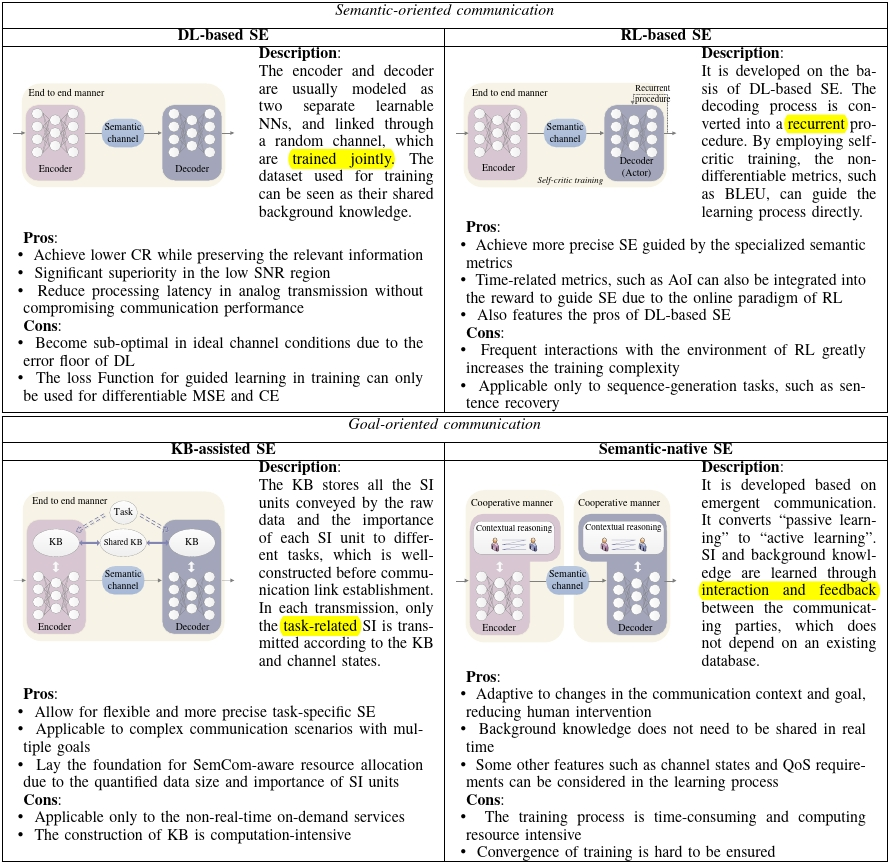
\includegraphics[width=0.7\textwidth]{assets/learning.jpg}
				\caption{Summary of generic semantic extraction methods \cite{Yang2022c}. ``CR'', ``SE'' and ``SI'' mean ``compression ratio'' and ``semantic extraction'' and ``semantic information''.}
			\end{figure}
			% ! semantic: meaning; task: goal (higher level) with more explicit object function
		\end{frame}
	\end{subsection}

	\begin{subsection}{Text Semantic}
		\begin{frame}{Text Semantic Metrics: BLEU}
			Word-Error Rate (WER) is not a good metric as two sentences with different wording can have high semantic similarity.
			\singlespacing
			BiLingual Evaluation Understudy (BLEU) \cite{Papineni2002} measures the similarity of the machine-translated text to a set of high quality reference translations
			\begin{equation}
				\log \text{BLEU} = \min (1 - \frac{l_{\hat{\boldsymbol{s}}}}{l_{\boldsymbol{s}}},0) + \sum_{n} u_n \log P_n
			\end{equation}
			\vspace{-0.3cm}
			\begin{itemize}
				\item $l_{\boldsymbol{s}}$ and $l_{\hat{\boldsymbol{s}}}$ are the word length of transmitted sentence $\boldsymbol{s}$ and received sentence $\hat{\boldsymbol{s}}$;
				\item $u_n$ is the weight of the $n$-gram;
				\item $P_n$ is the $n$-gram score (a function of the element frequency count);
				\item $\text{BLEU} \in [0,1]$: the higher the score, the higher similarity between the two sentences.
			\end{itemize}
		\end{frame}

		\begin{frame}{Text Semantic Metrics: Sentence Similarity}
			Semantic similarity \cite{Xie2021a} measures the semantic similarity level of two sentences
			\begin{equation}
				\tau(\hat{\boldsymbol{s}},\boldsymbol{s}) = \frac{B_{\Phi}(\boldsymbol{s}) B_{\Phi}(\hat{\boldsymbol{s}})^T}{\lVert B_{\Phi}(\boldsymbol{s}) \rVert \lVert B_{\Phi}(\hat{\boldsymbol{s}}) \rVert}
			\end{equation}
			\vspace{-0.3cm}
			\begin{itemize}
				\item $B_{\Phi}(\cdot)$ is the BERT model to map a sentence to its semantic vector space, which is a pre-trained model with billions of sentences;
				\item $\tau \in [0,1]$: the higher the score, the higher similarity between the two sentences.
			\end{itemize}
			% !  Instead of comparing two sentences directly, we compare their semantic vectors obtained by the BERT model
		\end{frame}

		\begin{frame}{Text Semantic Processing: DeepSC}
			\begin{figure}
				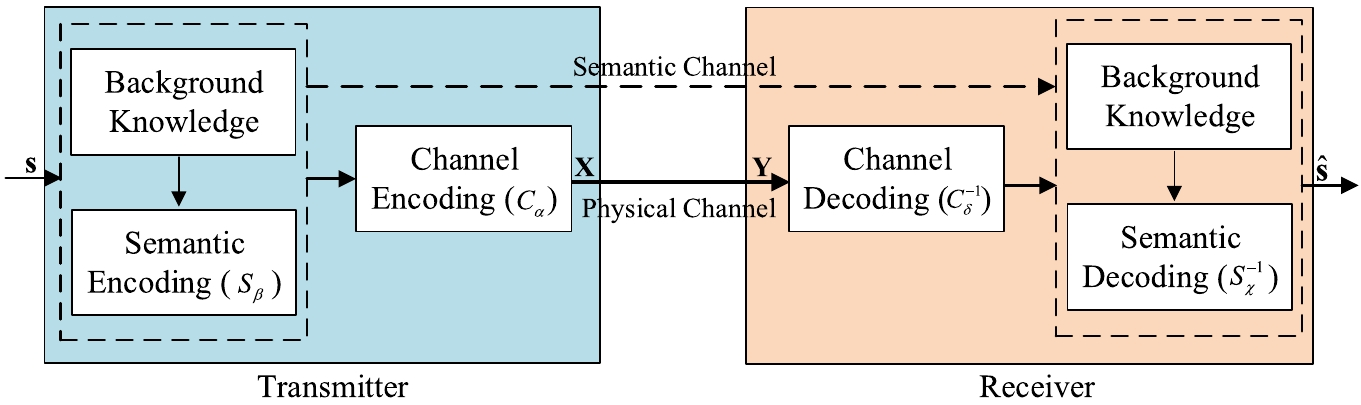
\includegraphics[width=\textwidth]{assets/deepsc.jpg}
				\caption{The framework of DL-enabled semantic text processing, DeepSC \cite{Xie2021a}.}
			\end{figure}
			\begin{itemize}
				\item Transmitter
				\begin{equation}
					\boldsymbol{X} = C_{\alpha}(S_{\beta}(\boldsymbol{{s}}))
				\end{equation}
				\item Receiver
				\begin{equation}
					\boldsymbol{Y} = \boldsymbol{H} \boldsymbol{X} + \boldsymbol{N}, \quad \hat{\boldsymbol{s}} = S_{\chi}^{-1}(C_{\delta}^{-1}(\boldsymbol{Y}))
				\end{equation}
				\item Physical channel: AWGN and fading
				\item Semantic channel: BLEU and sentence similarity
			\end{itemize}
		\end{frame}

		\begin{frame}{DeepSC: Transceiver Structure}
			\begin{figure}
				\subfloat[Transceiver structure]{
					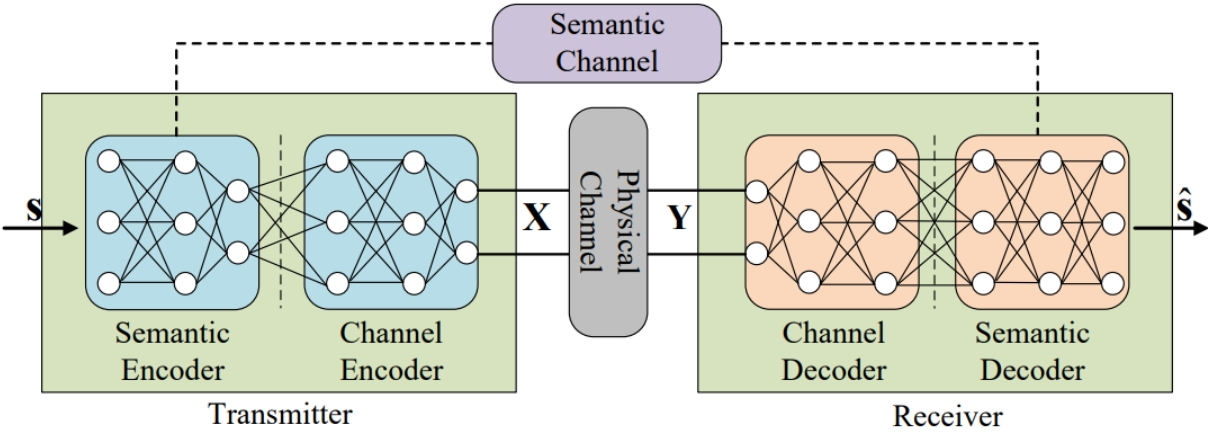
\includegraphics[width=0.75\textwidth]{assets/deepsc_transceiver.jpg}
				}
				\subfloat[Encoding example \cite{Xie2021a}]{
					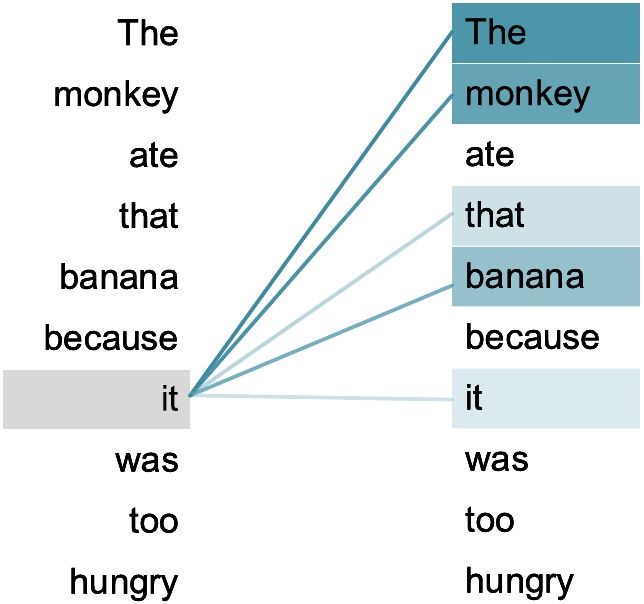
\includegraphics[width=0.25\textwidth]{assets/semantic_encoder_example.jpg}
				}
				\\
				\subfloat[Overall DNN \cite{Xie2021a}]{
					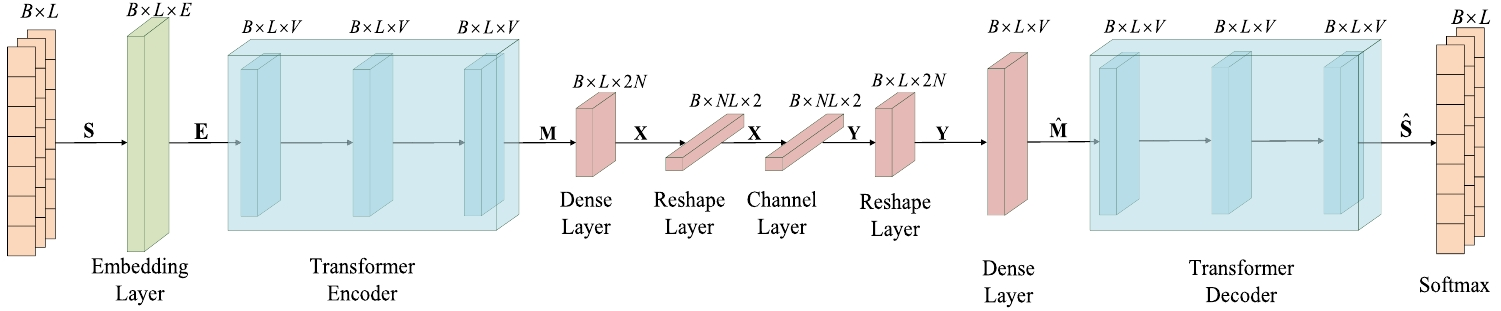
\includegraphics[width=\textwidth]{assets/deepsc_neural_network.jpg}
				}
			\end{figure}
			\vspace{-0.3cm}
			\begin{itemize}
				\item Merge the traditional and semantic communication into DNN
				\item Semantic encoder can learn the semantic in text
			\end{itemize}
		\end{frame}

		\begin{frame}{DeepSC: Training}
			\begin{figure}
				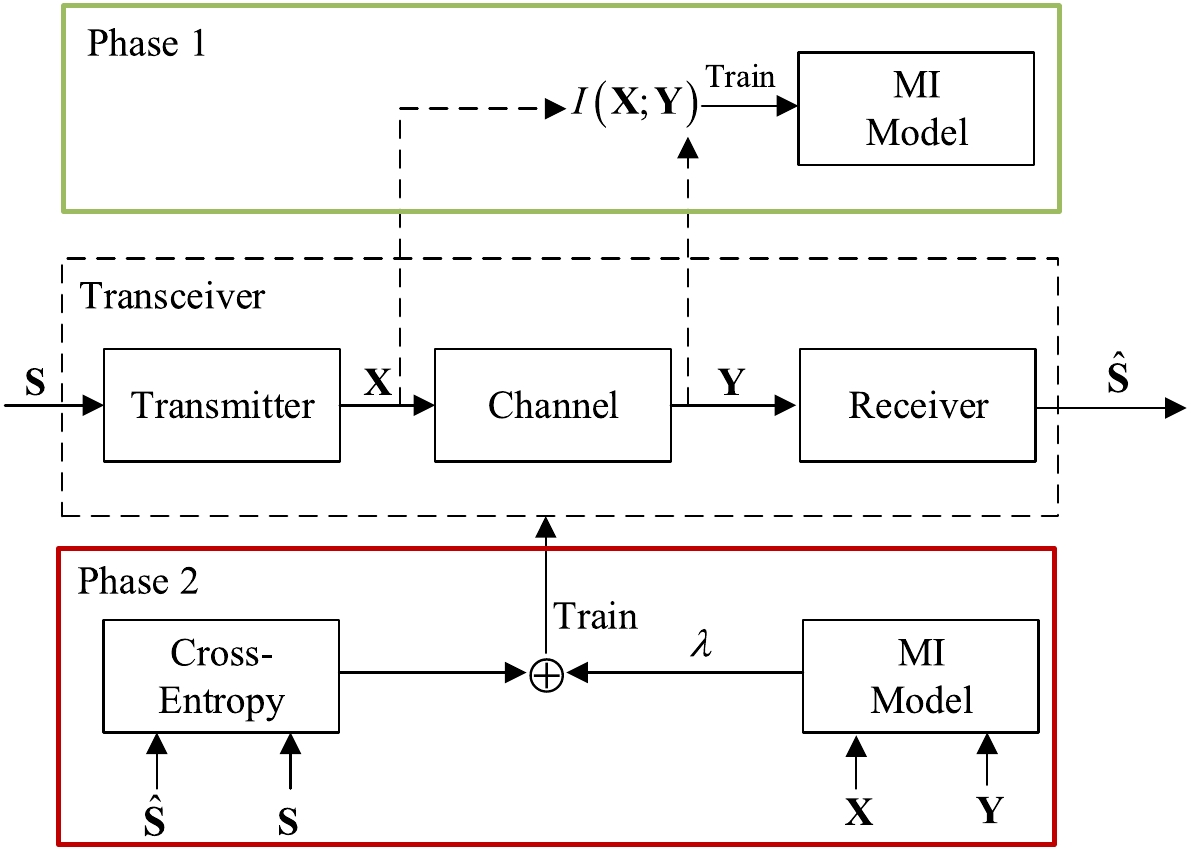
\includegraphics[width=0.6\textwidth]{assets/deepsc_training.jpg}
				\caption{Training framework of DeepSC \cite{Xie2021a}.}
			\end{figure}
			\begin{itemize}
				\item Phase 1 trains the mutual information estimation model
				\item Phase 2 trains the whole network based on the cross-entropy and mutual information
			\end{itemize}
		\end{frame}

		\begin{frame}{DeepSC: Simulation Results}
			Simulation setup:
			\begin{itemize}
				\item Dataset: The proceedings of the European Parliament
				\item Transmitter: 3 layers of Transformer encoder and 2 dense layers
				\item Receiver: 2 dense layers and 3 layers of Transformer decoder
			\end{itemize}
			\begin{figure}
				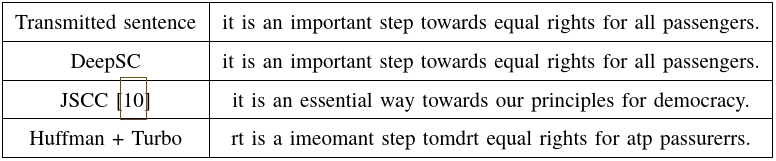
\includegraphics[width=\textwidth]{assets/deepsc_sentences.jpg}
				\caption{I/O sentences by DeepSC, LSTM-enabled joint source-channel coding \cite{Bourtsoulatze2019}, and conventional coding.}
			\end{figure}
		\end{frame}

		\begin{frame}{DeepSC: Simulation Results}
			\begin{figure}
				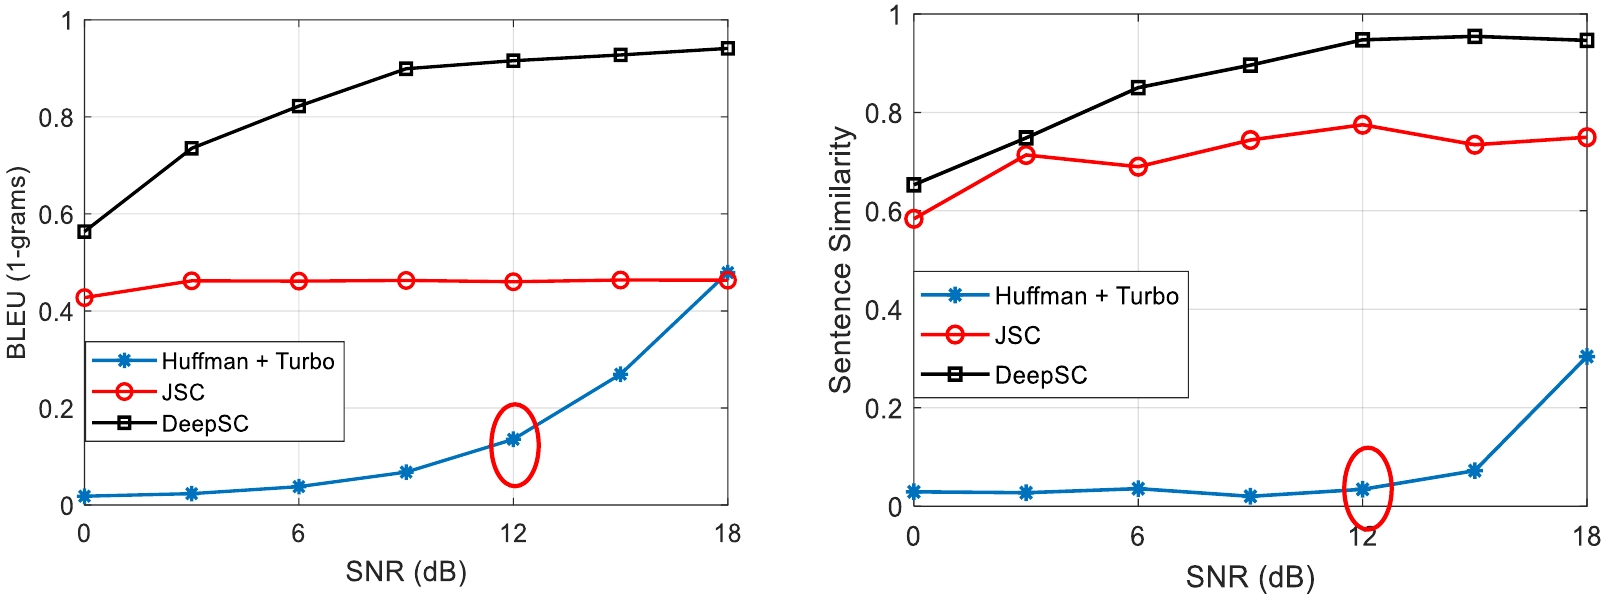
\includegraphics[width=\textwidth]{assets/deepsc_scores.jpg}
				\caption{BLEU and sentence similarity scores comparison.}
			\end{figure}
			\begin{itemize}
				\item All deep learning approaches are more competitive in the low SNR regime.
				\item The tendency in sentence similarity is much closer to human judgment:
				\begin{itemize}
					\item At $\text{SNR}=12$ dB, $20\%$ BLEU score $=$ approximate $0$ sentence similarity
					\item People are usually unable to understand the meaning of texts full of errors
				\end{itemize}
			\end{itemize}
		\end{frame}
	\end{subsection}

	\begin{subsection}{Image and Speech Semantic}
		\begin{frame}{Image and Speech Semantic Metrics}
			For image semantic, conventional metrics as peak signal-to-noise ratio (PSNR) and structural similarity index (SSIM), are often considered by engineers but fail to count many nuances of human perception.
			\singlespacing
			For speech semantic, the goal can be:
			\begin{itemize}
				\item Data reconstruction: involves the transmission and recovery of \emph{global} semantic information (e.g., voice of speaker, text information, delay)
				\item Speech synthesis: some semantic information (e.g., delay) can be omitted
			\end{itemize}
			\singlespacing
			For semantic communications serving different tasks, the performance metric is heavily dependent on the chosen ``semantic language'' for the application.
		\end{frame}

		\begin{frame}{Image Semantic: Simulation Results}
			\begin{figure}
				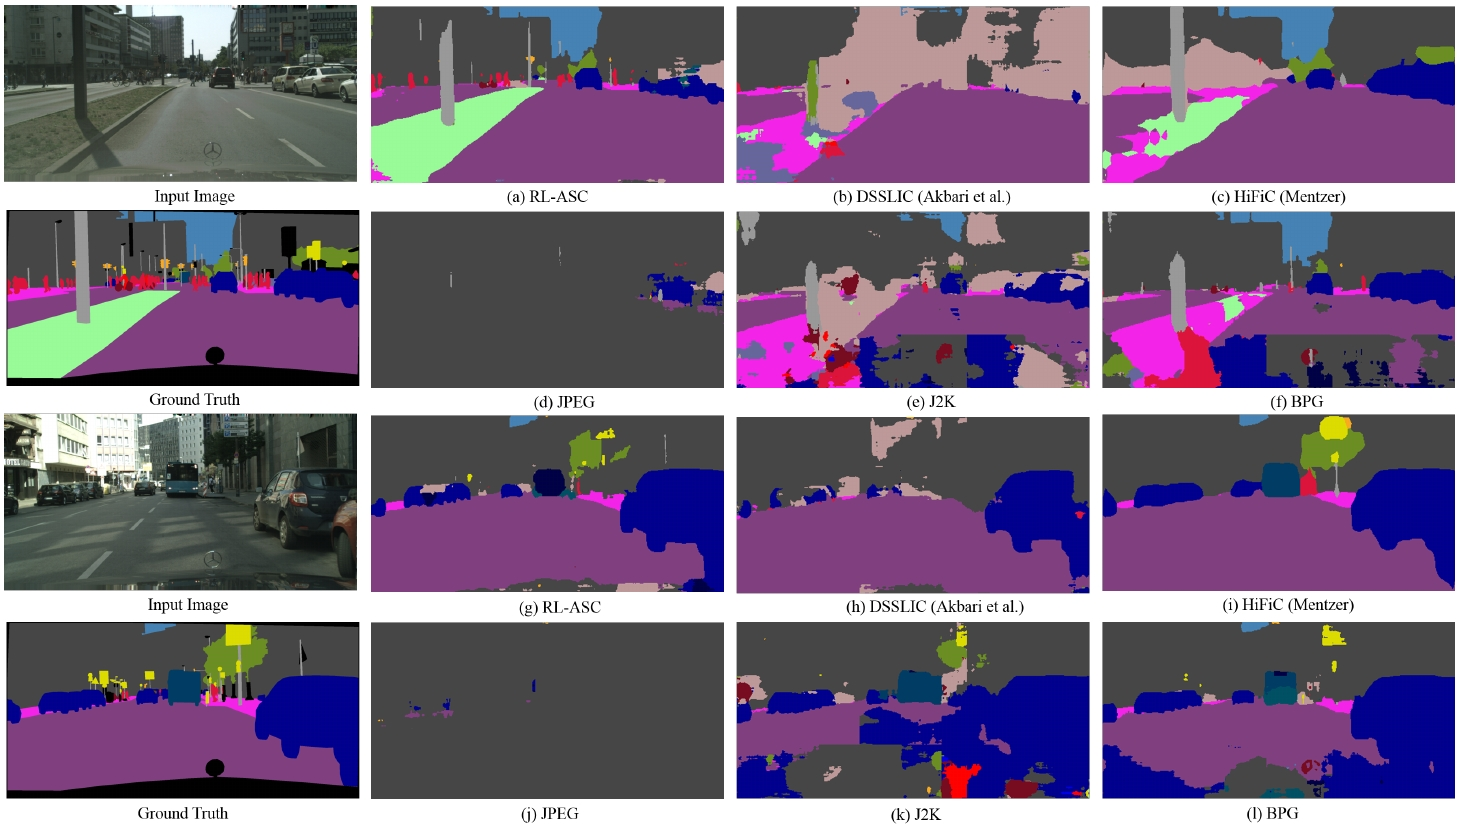
\includegraphics[width=\textwidth]{assets/semantic_image_example.jpg}
				\caption{Example of semantic image coding vs conventional learning and standard schemes \cite{Huang2022b}.}
			\end{figure}
		\end{frame}

		\begin{frame}{Image Semantic: Simulation Results}
			\begin{figure}
				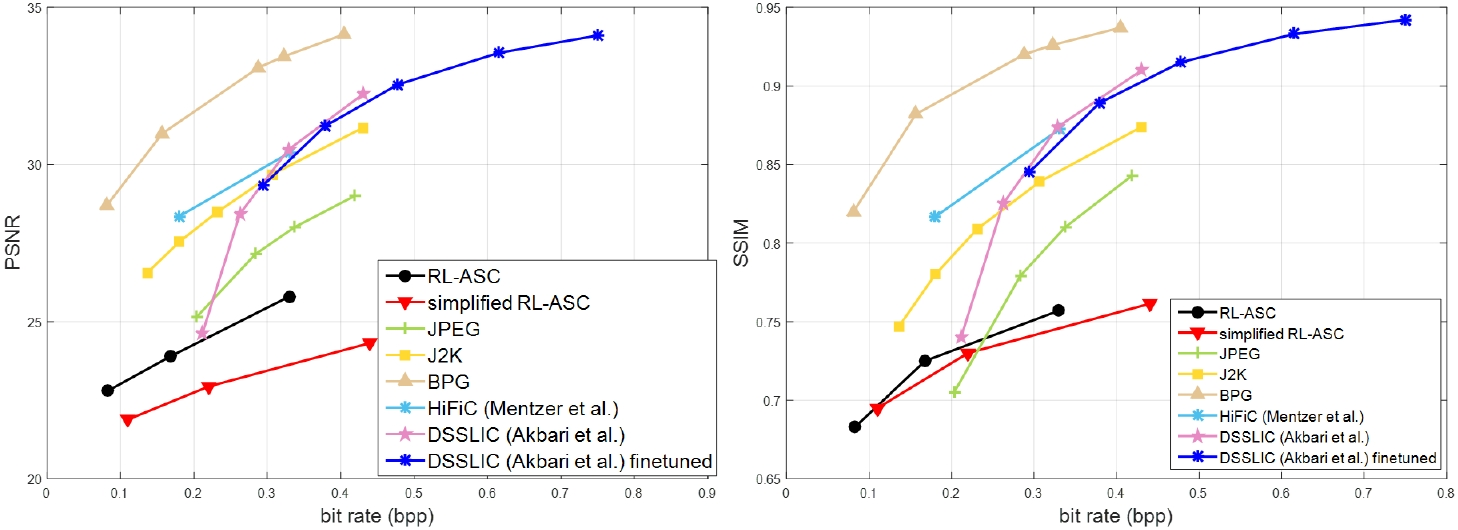
\includegraphics[width=\textwidth]{assets/semantic_image_performance.jpg}
				\caption{The rate-distribution performance in terms of PSNR and SSIM \cite{Huang2022b}. Higher value means better performance.}
			\end{figure}
			\begin{itemize}
				\item The baselines achieve better performance since they are optimized w.r.t. both metrics;
				\item The proposed RL-ASC is tolerable to pixel errors and does not attempt to ensure local consistency;
				\item Disparity and tradeoff between the pixel-level loss and the semantic loss!
			\end{itemize}
		\end{frame}

		\begin{frame}{Speech Semantic: Simulation Results}
			\begin{figure}
				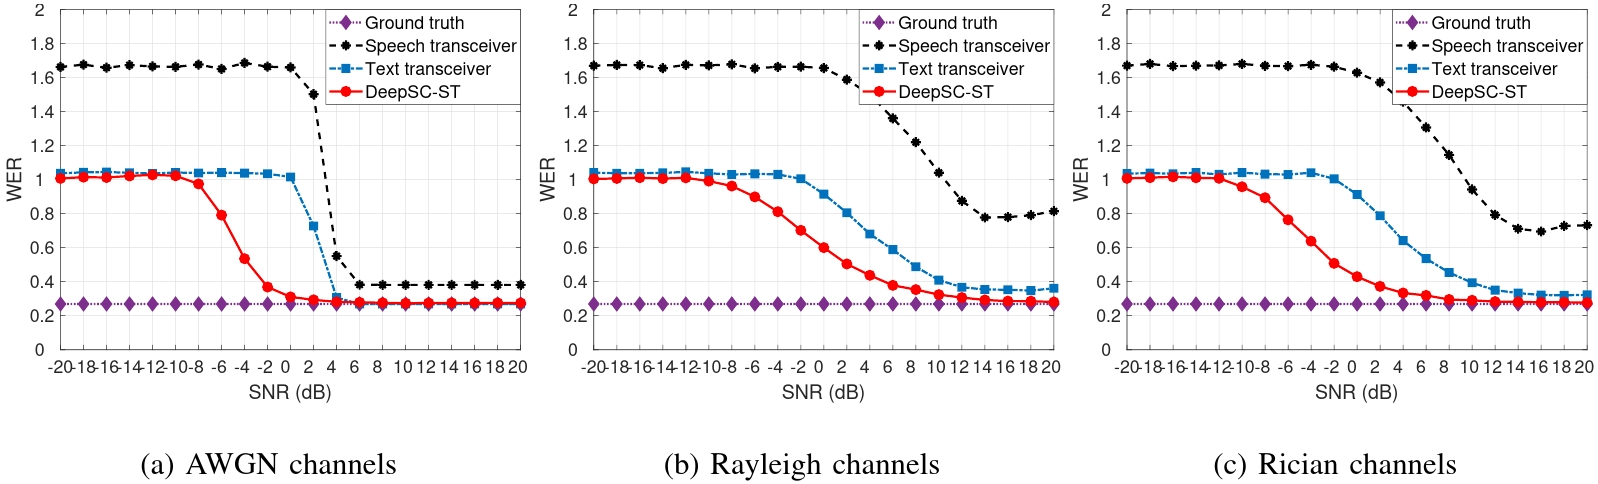
\includegraphics[width=\textwidth]{assets/semantic_speech_performance.jpg}
				\caption{Word-error rate vs SNR for speech transceiver, text transceiver, and DeepSC-ST (speech transmission) \cite{Weng2022}.}
			\end{figure}
			\begin{itemize}
				\item DeepSC-ST provide lower WER under various channel conditions;
				\item Performance gap is large at low SNR.
			\end{itemize}
		\end{frame}
	\end{subsection}
\end{section}

\begin{frame}{Challenges}
	Semantic communication is ``beyond Shannon'' with many open issues:
	\begin{itemize}
		\item \textbf{Semantic theory:} can we follow the conventional path to quantify semantic communications (e.g., entropy, channel capacity, rate-distribution theory, and the relationship between inference accuracy and transmission rate)?
		\item \textbf{Semantic transceiver:} how to design a general semantic joint source and channel coding for different types of sources? how to define a general semantic noise?
		\item \textbf{Semantic comms with reasoning:} how to enable reasoning, planning, and handling exceptions? how much benefit is obtainable?
		\item \textbf{Resource allocation in semantic comms:} how to evaluate semantic communication efficiency (i.e., semantic transmission rate or semantic spectral efficiency)? how to formulate a general resource allocation problem?
		\item \textbf{Semantic performance metrics:} how to evaluate the amount of semantic information that has been preserved or missed (i.e., semantic error rate)?
		\item \textbf{Semantic applications:} what are the potential killing applications (e.g., video conference)?
	\end{itemize}
\end{frame}

\begin{frame}{Thank You!}
	\begin{figure}
		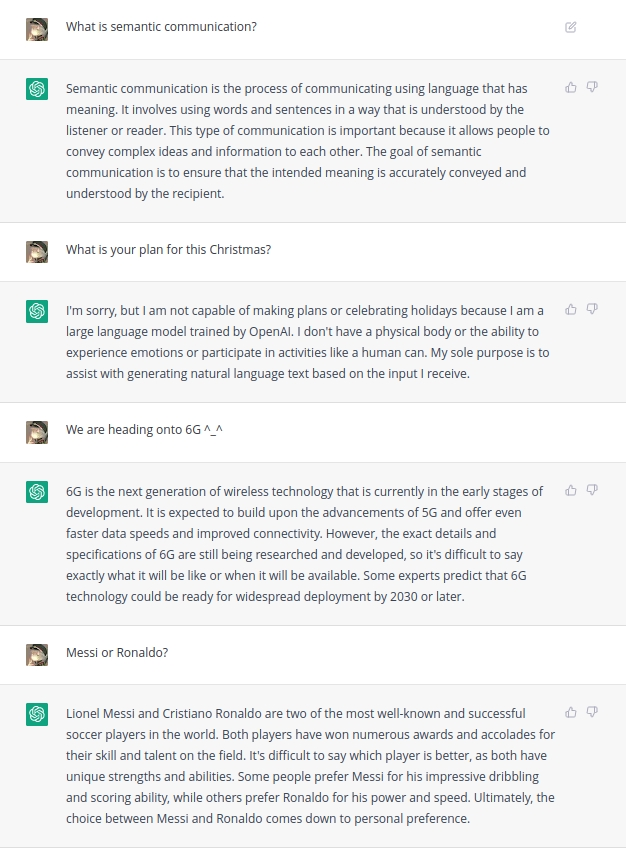
\includegraphics[width=0.52\textwidth]{assets/chatgpt.jpg}
	\end{figure}
\end{frame}

\bibliographystyle{IEEEtran}
\bibliography{IEEEabrv,library.bib}
\end{document}
